%% LaTeX-Beamer template for KIT design
%% by Erik Burger, Christian Hammer
%% title picture by Klaus Krogmann
%%
%% version 2.1
%%
%% mostly compatible to KIT corporate design v2.0
%% http://intranet.kit.edu/gestaltungsrichtlinien.php
%%
%% Problems, bugs and comments to
%% burger@kit.edu

\documentclass[18pt]{beamer}
\usepackage[utf8x]{inputenc}
\usepackage{units}
\usepackage{booktabs}

%% CUSTOM
\usepackage{amsmath}
\usepackage{algpseudocode}

%% Definitions
\DeclareMathOperator{\div2}{div}
\renewcommand{\algorithmicrequire}{\textbf{Input:}}
\renewcommand{\algorithmicensure}{\textbf{Output:}}
\algnewcommand\algorithmicto{\textbf{to}}
\algrenewtext{For}[3]{\algorithmicfor\ $#1 \gets #2$ \algorithmicto\ $#3$ \algorithmicdo}
\algnewcommand\algorithmicod{\textbf{od}}
\algrenewtext{EndWhile}{\algorithmicod}
\algrenewtext{EndFor}{\algorithmicod}
%\AtBeginSection[]{%
%\begin{frame}<beamer> % do nothing in handouts
%    \frametitle{Überblick}
%    \tableofcontents[sectionstyle=show/shaded,
%    subsectionstyle=show/show/hide]
%\end{frame}
%}
%\AtBeginSubsection[]{%
%\begin{frame}<beamer> % do nothing in handouts
%    \frametitle{Überblick}
%    \tableofcontents[sectionstyle=show/shaded,
%    subsectionstyle=show/shaded/hide]
%\end{frame}
%}

%% SLIDE FORMAT

% use 'beamerthemekit' for standard 4:3 ratio
% for widescreen slides (16:9), use 'beamerthemekitwide'

\usepackage{templates/beamerthemekit}
%\usepackage{templates/beamerthemekitwide}

 %% TITLE PICTURE

 % if a custom picture is to be used on the title page, copy it into the 'logos'
 % directory, in the line below, replace 'mypicture' with the 
 % filename (without extension) and uncomment the following line
 % (picture proportions: 63 : 20 for standard, 169 : 40 for wide
 % *.eps format if you use latex+dvips+ps2pdf, 
 % *.jpg/*.png/*.pdf if you use pdflatex)


 \titleimage{banner}
 
 
%% Define some colors:
\definecolor{darkblue}{rgb}{0,0,.5}
\definecolor{darkgreen}{rgb}{0,.5,0}

 %% TITLE LOGO

 % for a custom logo on the front page, copy your file into the 'logos'
 % directory, insert the filename in the line below and uncomment it

\titlelogo{logo_150x150}
 
 % (*.eps format if you use latex+dvips+ps2pdf,
 % *.jpg/*.png/*.pdf if you use pdflatex)
 
 %% TikZ INTEGRATION
 
 % use these packages for PCM symbols and UML classes
 % \usepackage{templates/tikzkit}
 % \usepackage{templates/tikzuml}
 
 % the presentation starts here
 
\author{Dominik Muth - dominik.muth@student.kit.edu}
\institute{Institut f\"ur Informatik}

\subtitle{Foliensatz 14}
\date{7. Februar 2013}

\newcommand{\sq}{$\square$}
\newcommand{\da}{$\downarrow$}
\DeclareMathOperator{\cod}{cod}

\begin{document}

\begin{frame}
    \titlepage
\end{frame}

\begin{frame}{Outline/Gliederung}
    \tableofcontents
\end{frame}

\section{Statistik}
\begin{frame}{Statistiken}
    Die folgenden Grafiken beziehen sich
    \begin{itemize}
        \item bei den Übungsblättern auf diejenigen, die den Übungsschein erhalten haben und
        \item bei der Übungsklausur auf diejenigen, die abgegeben haben.
    \end{itemize}
\end{frame}
\begin{frame}{Verlauf des Punktestands}
    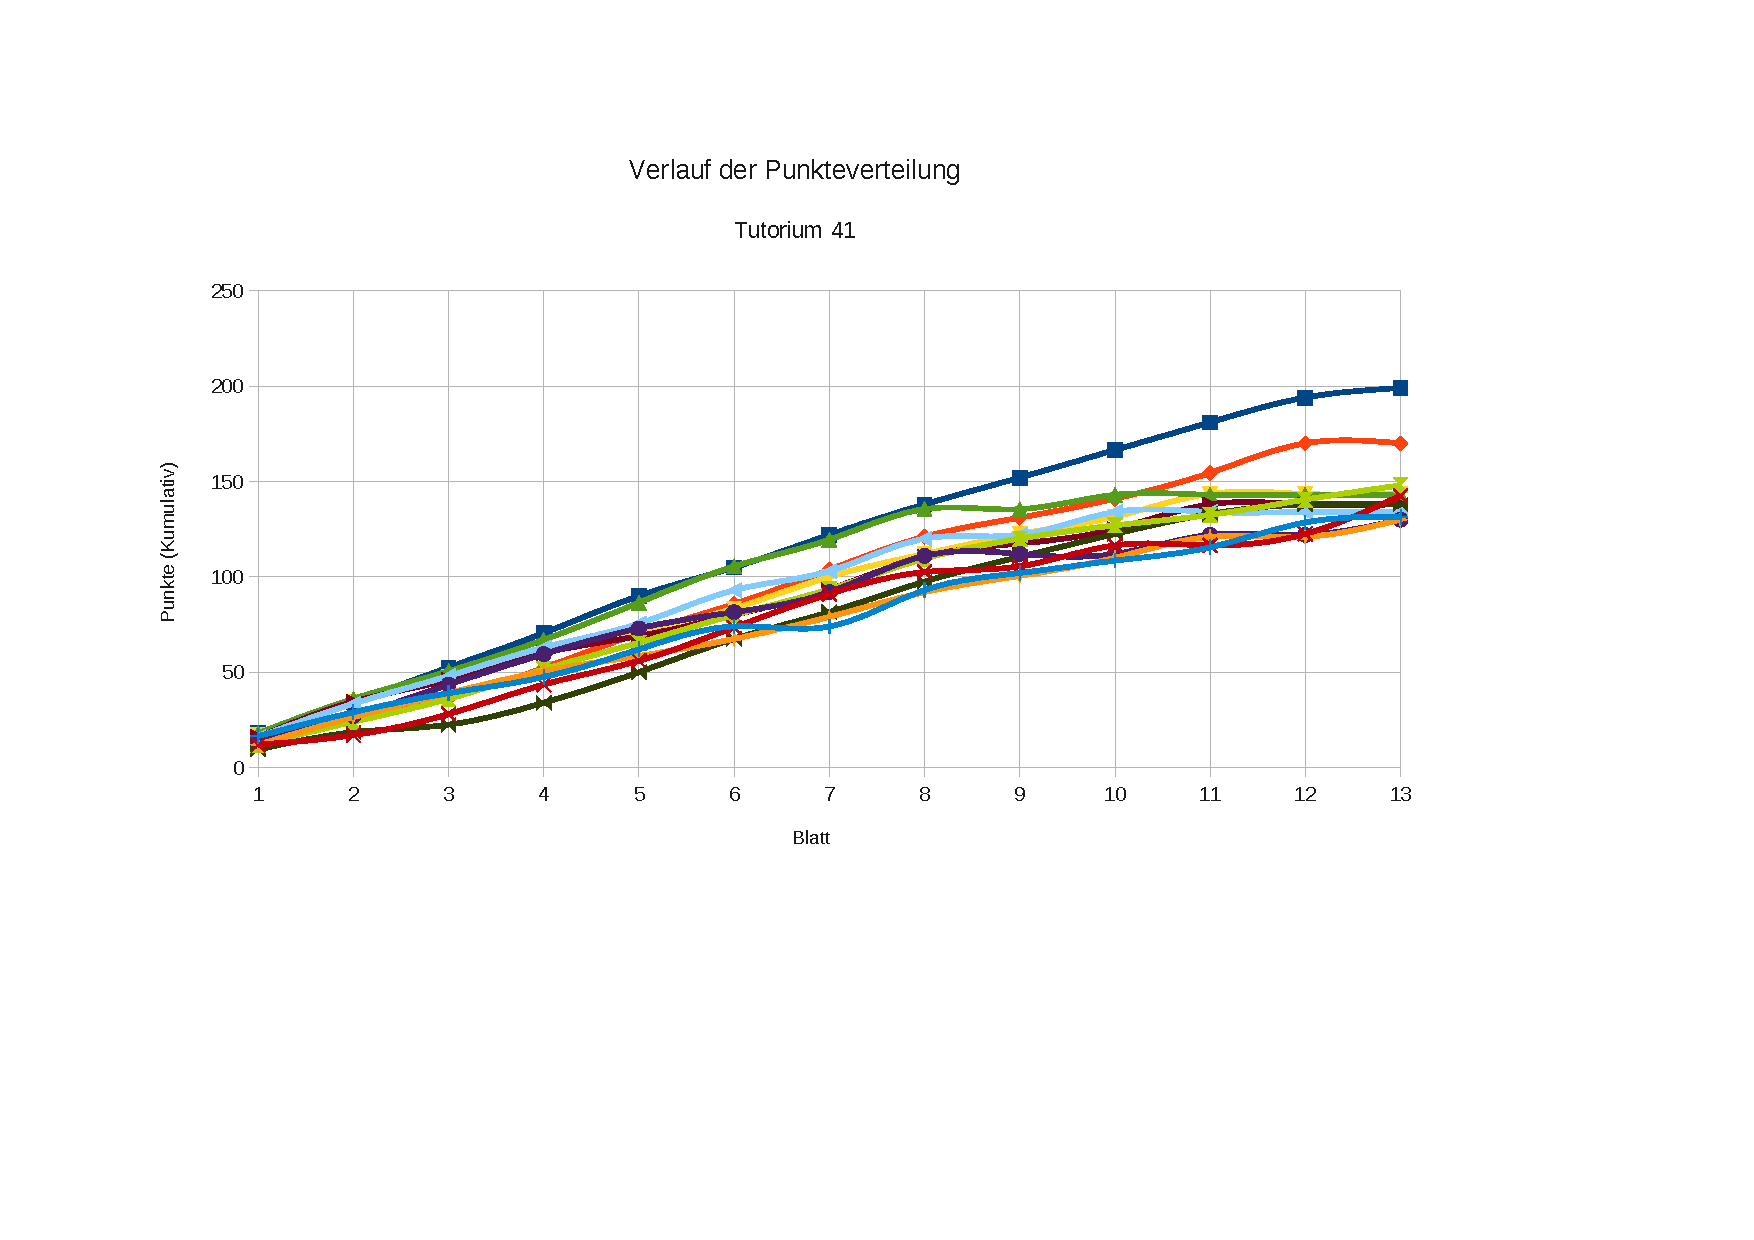
\includegraphics[scale=0.4]{graphics/14/punkte1.pdf}
\end{frame}
\begin{frame}{Verlauf des Punktestands}
    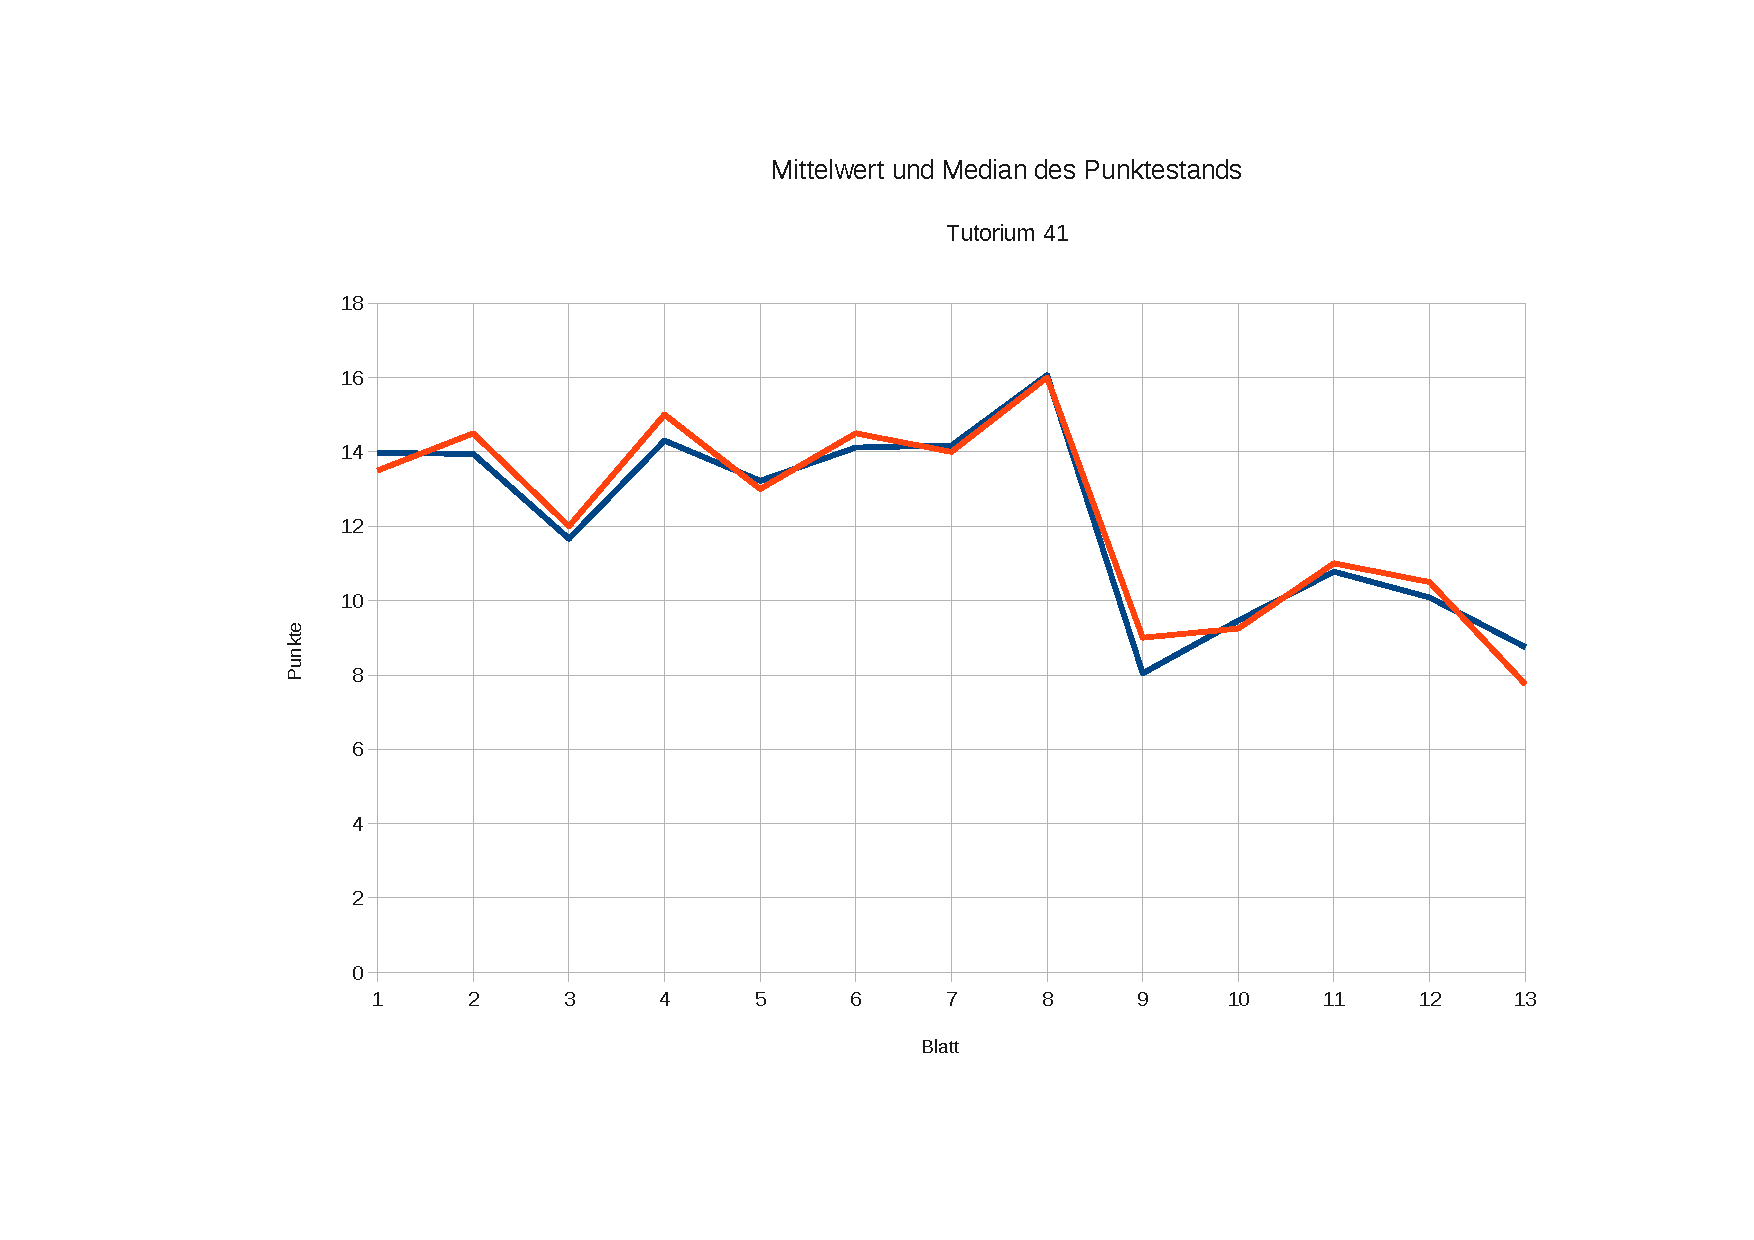
\includegraphics[scale=0.35]{graphics/14/punkte2.pdf}\\
    blau: Mittelwert, rot: Median
\end{frame}
\begin{frame}{Punkteverteilung in der Probleklausur}
    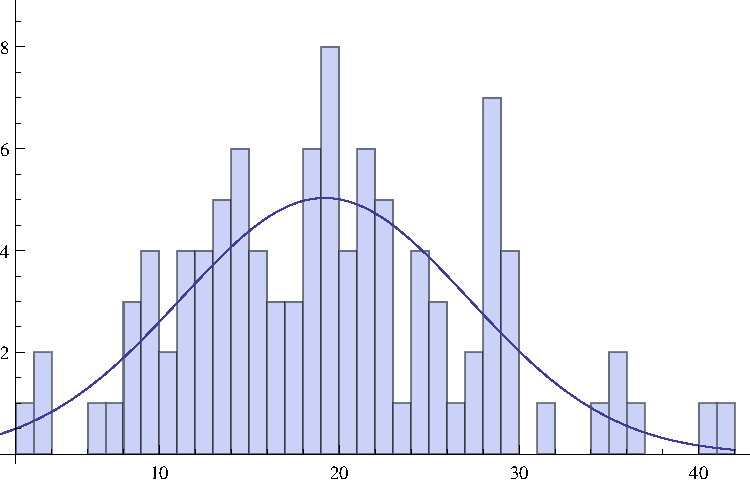
\includegraphics[scale=0.9]{graphics/14/probeklausur1.pdf}
\end{frame}
\section{Wiederholung}
\begin{frame}{Wiederholung - Quiz}
    \begin{itemize}
        \item Jedes Problem kann von einer Turingmaschine entschieden werden. \visible<2>{Nein.}
        \item Warum? \visible<3>{Siehe Halteproblem.}
        \item Gilt $\mathrm{P} \subset \mathrm{PSPACE}$? \visible<4>{Ja.}
        \item Gibt es endliche Akzeptoren für Sprachen $L$, die weniger Zustände haben als $L$ Nerode-Äquivalenzklassen? \visible<5>{Nein.}
    \end{itemize}
\end{frame}
\section{Kongruenzrelationen}
\begin{frame}{Verträglichkeit}
    \begin{block}{Definition: Verträglichkeit}
        Es sei $\equiv$ eine Äquivalenzrelation auf einer Menge $M$ und $f: M\rightarrow M$ eine Abbildung. Man sagt, dass $\equiv$ mit $f$ verträglich ist, wenn für alle $x_1, x_2 \in M$ gilt:
        \begin{align*}
            x_1 \equiv x_2 \Longrightarrow f\left( x_1 \right) \equiv f\left( x_2 \right)
        \end{align*}
    \end{block}
    Was bedeuted das anschaulich? Fallen euch Beispiele ein?
\end{frame}
\begin{frame}{Beispiel modulo n}
    Wir kennen noch vom letzten Mal:
    \begin{align}
        x_1 \equiv x_2 \left( \mod n \right) \Leftrightarrow x_1 -x_2 = kn\label{eq1}
    \end{align}
    \pause
    Das heißt auch, dass $x_1$ und $x_2$ bei einer Division mit $n$ den gleichen Rest haben.
    \pause
    \begin{align}
        y_1 \equiv y_2 \left( \mod n \right) \Leftrightarrow y_1 - y_2 = mn\label{eq2}
    \end{align}
    \pause
    Ich behaupte es gilt:
    \begin{align}
        x_1 + y_1 \equiv x_2  + y_2 \left( \mod n \right)\label{rel1}\\
        x_1 \cdot y_1 \equiv x_2 \cdot y_2 \left( \mod n \right)\label{rel2}
    \end{align}
    Beweis.
\end{frame}
\begin{frame}{Beweis von \eqref{rel1}}
    Addieren nun die beiden Gleichungen \eqref{eq1} und \eqref{eq2}:
    \pause
    \begin{align*}
        \left( x_1 + y_1 \right) - \left( x_2 + y_2 \right) = \left( x_1 - x_2 \right) + \left( y_1 - y_2 \right) = \left( k + m \right) n
    \end{align*}
    \pause
    Und wir sehen, dass gilt
    \begin{align*}
        x_1 + y_1 \equiv x_2 + y_2 \left( \mod n \right)
    \end{align*}
\end{frame}
\begin{frame}{Beweis von \eqref{rel2}}
    Löse Gleichung~\eqref{eq1} nach $x_1$ auf und Gleichung~\eqref{eq2} nach $y_1$ und multipliziere beide Seiten:
    \begin{align*}
        x_1 \cdot y_1 &= \left( x_2 + kn \right) \cdot \left( y_2 + mn \right)\\
                        &= x_2 \cdot y_2 + n\left( mx_2 + ky_2 + kmn \right)\\
        x_1 \cdot y_1 - x_2 \cdot y_2  &= n\left( mx_2 + ky_2 + kmn \right)\\
            \Longleftrightarrow x_1\cdot y_1 &\equiv x_2 \cdot y_2 \left( \mod n \right)
    \end{align*}
\end{frame}
\begin{frame}{Kongruenz}
    Damit können wir auch ``nur mit Repräsentanten'' der Äquivalenzklasse rechnen:
    \begin{align*}
        [2] + [3] = [2 + 3] = [5] = [0]\\
        [2] \cdot [3] = [2 \cdot 3] = [6] = [1]\\
    \end{align*}
    Nennt weitere Beispiele für die Äquivalenzrelation Kongruent Modulo $i$, wobei sich $i$ bei jedem von euch erhöht.
\end{frame}
\begin{frame}{Verträglichkeit und Kongruenzrelationen}
    Die Operationen $+$ und $\cdot$ sind also verträglich mit unserer Relation ``kongruent modulo n''.\\
    \begin{block}{Definition: Kongruenzrelation}
        Eine Funktion, die mit allen gerade interessierenden Funktionen oder/und Operationen verträgich ist, nennt man auch \emph{Kongruenzrelation}.
    \end{block}
\end{frame}
\begin{frame}{Kongruenz und die Nerode-Äquivalenz}
    Gegeben sei die Funktion:
    \begin{align*}
        f_x': A_{/\equiv_L}^* \rightarrow A_{/\equiv_L}^*: [w]\mapsto [wx]
    \end{align*}
    Warum ist die Nerode-Äquivalenz mit dieser Abbildung verträglich?
    \visible<2>{Gegeben sei $w_1\equiv_L w_2$, das heißt nach Definition der Nerode-Äquivalenz:
        \begin{align*}
            w_1 w \in L &\Leftrightarrow w_2 w \in L\\
            \left( w_1 x \right) v \in L &\Leftrightarrow w_1\left( x v \right) \in L\\
            &\Leftrightarrow w_2\left( x v \right) \in L \text{ weil } w_1 \equiv_L w_2\\
            &\Leftrightarrow \left( w_2 x \right)v \in L
        \end{align*}
    Damit ist gezeigt, dass die Nerode-Äquivalenz mit der Konkatenation verträglich ist.}
\end{frame}
\begin{frame}{Induzierte Operationen}
    Wir wissen nun, dass $f_x : A^*:w\mapsto wx$ (Konkatenation) mit $\equiv_L$ (Nerode-Äquivalenz) verträglich ist. Damit gilt auch:
    \pause
    \begin{align*}
        f'_x : A_{/\equiv_L}^* \rightarrow A_{/\equiv_L}^*:[w]\mapsto[wx]
    \end{align*}
    Was heißt das?\\
    \pause
    Die Nerode-Äquivalenz ist mit der Konkatenation verträglich. Damit ergibt sich auch eine Relation auf die Äquivalenzmenge $A_{/\equiv_L}^*$. (Die obige Funktion ist \emph{wohldefiniert}.)\\
    \pause
    Damit können wir uns einen endlichen Akzeptor konstruieren, wähle:
    \begin{itemize}
        \item $z_0 = [\varepsilon]$ (Startzustand) und
        \item $F = \left\{ [w] | w\in L \right\}$ (akzeptierte Zustände)
    \end{itemize}
\end{frame}
\section{Halbordnungen}
\begin{frame}{Antisymmetrie}
    \begin{block}{Definition: Antisymmetrie}
        Eine Relation $R\subseteq M\times M$ heißt \emph{antisymmetrisch}, wenn für alle $x, y \in M$ gilt:
        \begin{align*}
            xRy \wedge yRx \Rightarrow x=y
        \end{align*}
    \end{block}<++>
\end{frame}<++>
\end{document}
